% !TEX root = ../disertace.tex
%!TEX encoding = UTF-8 Unicode

\chapter{S-Data}
\label{sec:s}
\section{Introduction}
\label{sec:s:intro}
When we faced the prospect of creating annotations of MWEs in the PDT, we already knew that we want to work with t-layer, as described in \Sref{sec:intro:motiv}. We were however reluctant to add our data directly into t-files. The principal reason was our uncertainty, whether this information really belongs to the tectogrammatical layer of description. There were also secondary, but all the more practical reasons: the t-files are rather complex and we wanted a simple way to isolate our annotations. Also, we prefer to keep the stable PDT 2 as is and clearly separate our experiments from this stable data. 

That is why we decided to create a stand-off layer for any additional annotations that use nodes of a tree and creates some new units, while linking these new units to entries from some annotation lexicon. Since PDT 2 uses the PML format, our obvious choice was to design an additional PML layer.

\section{PML -- Prague Markup Language}
\label{sec:pml}
PML is a language designed by \citet{pajas:2005} for structured linguistic annotation. It can be used equally well for speech data \citep{hajic:2008}, text corpora annotated using dependency syntax, phrase-structure trees, or even both together as different layers of annotation over single underlying data (cf. \citealp{cinkova:2009}). Dictionaries can also be represented in PML, e.g. PDT-Vallex -- the valency dictionary that is a part of the PDT 2.0 \citep{pdtvallex:2003a}.

PML is a XML language, which means it can take advantage of the rich existing XML tools, above else parsers and validators. PML itself however defines in addition many data types and a system of roles. To allow for efficient design and validation of PML files, there is PML Schema. PML Schema files themselves can be validated using RelaxNG. The schema of PML workflow is illustrated in \Fref{fig:pml}. The full set of tools for working with PML data was published as the PML Toolkit \citep{pajas:2009}.

\begin{figure}[htbp]
   \centering
   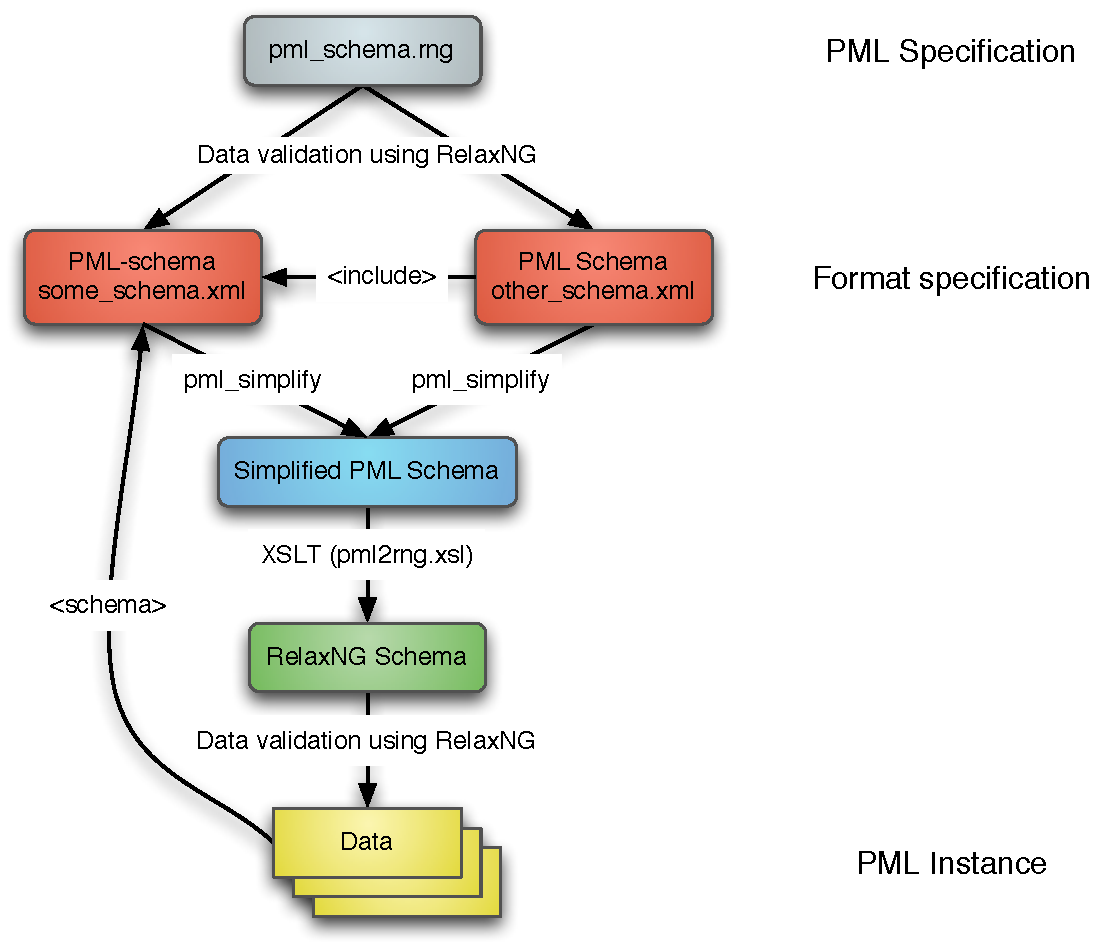
\includegraphics[width=0.9\textwidth]{images/pml-schema.pdf}
   \caption{A schema of a PML workflow. It does not illustrate all the possible interactions of PML data and schema files.}
   \label{fig:pml}
\end{figure}

\section{The design and the PML schema of \sdata}
\label{sec:s:design}
\sdata\ means s-layer PML files and the PML schema of these files. The idea behind \sdata\ design is to have a simple way to store additional ``sense'' annotations over any layer of PDT. The annotations are stored as a set of ``sense'' nodes. Each s-node contains a link to a sense repository (annotation lexicon) and a set of references to nodes (m-, a- or t-) that correspond to an instance of the sense. An \sf\ is thus basically a very simple flat list of \sn{}s. It does not contain any trees. A single \sf\ can only reference a single PDT file: either tectogrammatical, or analytical, or even morphological layer can be used, but references to different layers cannot be mixed in one s-file.

The design of \sdata\ is quite universal. S-files can be used to provide additional annotations over any PML files that contain nodes thati have an attribute ID. The sense repository (annotation lexicon) can be any dictionary that provides IDs for the entries. The tools used in our annotations mostly expect PDT PML or the particular \sf{}s that we have used, but that is mostly for convenience. Should the need appear to adapt the workflow a different corpus represented by PML files and a different annotation lexicon, the changes required would be rather minor.



\section{Visualisation}
\label{sec:s:visual}
There are two basic ways to view st-nodes: in \seman\ or in \tred. Both of these need to use the ``t-a-m-w-'' PDT files to display the sentence and/or the tree for each sentence and then they read the \stf\ to add the information about \stn{}s. The \stn{}s are displayed as colour boxes or bubbles over the words in a sentence or nodes in a tree in \seman\ or \tred\ respectively.

PML-TQ server may seem like an obvious third choice for the visualisation, but currently it is not the case. Since PML-TQ server uses \tred\ for the visualisation of trees, the SVG graphic representation of a tree in PML-TQ client is actually generated by \btred\ server running on the PML-TQ server. The problem is that \tred\ does  currently use bitmap patterns in addition to colours to distinguish between node groups. The patterns are then not exported into SVG and the result is that in our particular annotation we can see only partial information. While keeping the distinction of NE types and \semlex\ entries, we loose the information on annotators. There is also no easy way to tell whether the extent of the node group is correct, because in case annotators disagreed and one annotated nodes AB and the other BC, the node groups would merge into ABC. That is why currently, until for instance opacity is used to represent the information from patterns during SVG export in \tred, PML-TQ server is not a suitable visualisation tool for our annotations. 

\subsection{Visualisation using \seman}
The visualisation of annotated files in \seman\ has the advantage of showing whole text with all the \mwe{}s clearly marked in a single glance. Integration of the SemLex browser is also beneficial, because it allows fast and convenient lookup of annotated \mwe{}s in \seman. Details of \seman\ interface are described in \Sref{sec:seman}. 

There are, however, also some drawbacks of this ``full plain text of an article'' approach: \xxx{dokoncit}
\subsection{Visualisation using \tred}
\todo

\section{\tred\ extension}
\label{sec:s:ext}

\tred\ has a powerful mechanism that allows it to be extended for new tasks. We developed an extension \texttt{pdt-t-st} that allows to see MWEs as graphically marked groups of tectogrammatical nodes. 

 Main features of the extension:
 \begin{itemize}
\item
Merges the \stf{}s into \tf{}s and allows to display these enriched tectogrammatical trees.
\item
Types of annotated MWEs (i.e. types of NEs and \semlex\ entries) are distinguished with the same colours that were used in \seman\ during annotations. This allows not only for easily seeing NE types, but also easily spotting annotators' disagreement on them. 
\item
Allows to merge annotations of several annotators into one \tf. 
\item
Each annotator's MWEs have a unique raster. It is thus easy to spot annotators' partial or full disagreement not on types of MWEs, but also on their spans.
\end{itemize}

 There are two ways to merge the \sdata\ and \tdata: 
 \begin{enumerate}
\item
Merge on opening the \stf\ in \tred, and
\item
Static merge that produces the merged \verb=*.t.mwe.gz= file. 
\end{enumerate}
The dynamic merging is done using a newly developed feature of \tred\footnote{Developed by Petr Pajas} that allows to apply arbitrary perl transformations on the input data. Thus we open the \stf, use the mechanism of extensions to activate our extension by identifying the \stf\ as data the extension can process and call our transformation. The transformation requires a \tf\ annotated by this \sf\ to be present in the same directory. The \tf\ and \sf\ are parsed, and for each \stn\ we find a tectogrammatical tree that includes \tn{}s annotated (i.e. referenced) in this \stn. When we have a root of the correct t-tree, the \stn{}s are basically added into an attribute \texttt{mwes} of this t-root. The attribute is rather complex, because it contains lists of \stn{}s for all annotators that annotated any \stn{}s in this tree. Some small transformations of \stn{}s are needed, as well as creation of some new XML nodes, to represent the information from \sf{}s in the \tf{}s properly. For all the details inspect the code of \verb=<tred-extensions-dir>/pdt_t_st/libs/SDataMerge.pm=.

\todo\ \xxx{Doplnit, co je v extenzi, jak extenze bojuje o to, aby dostala ``svoje'' data prave ona (ten podivny nedokumentovany hack). Doplnit, jak funguje exekuce a jak nadvakrat se to zatim dela, kdyz chci mit soubor s anotacemi dvou anotatoru.}